

%\documentclass[aip,reprint]{revtex4-1}
%\documentclass[sn-mathphys]{sn-jnl}
\documentclass[10pt]{iopart}
%\documentclass[aip,jap,preprint]{revtex4-1}
\usepackage{graphicx}% Include figure files
\usepackage{dcolumn}
\usepackage{color}
\usepackage{color,soul}
%\draft % marks overfull lines with a black rule on the right

\begin{document}
Dear Editor,

We like to express our appreciation to the reviewers for their comments.
We are resubmitting the revised version of the paper number SST--108576.
We have studied the comments of the reviewer carefully, and have changed the text according to the comments they
have listed.
The location of revisions is  highlighted by yellow in ``Marked--SST--108576.pdf''.
Below we refer to each of the reviewer’s comments.



\subsection*{Response to Reviewer \#1 }

\noindent
\textcolor[rgb]{0.00,0.50,1.00}{\textbf{Comment~1.}}
\emph{Details that how the microwave treatments affect the semiconductors are not clear.
The author claimed that it was not only heating up, and several possibilities were suggested.
But still the physics of the microwave treatment is very unclear for the reviewer.}

\noindent
\textcolor[rgb]{0.51,0.00,0.00}{\textbf{Reply:}}
Let's consider the possible ways microwave treatments affect defects in structures under investigation.
The primary process, which determines defect production under irradiation,
is a displacement of the atoms from the sites of the lattice.
But the energy of a photon with frequency 2.45~GHz is about $10^{-5}$~eV only;
the threshold displacement energies in GaAs and SiC are (8-28)~eV \cite{Ed:GaAs} and (20-35)~eV \cite{Ed:SiC}, respectively.
Therefore such a channel of microwave-induced modification of defect subsystem is unreal.

Microwave energy is known to transform into heat inside the material.
Processes based on microwave heating find many industrial applications.
But the used experimental procedure
(pulsed microwave radiation with a period of 500~s and a duty cycle of 1\%)
allowed prevention of essential heating.
The calculation according to Bacherikov~\emph{et al}. \cite{Bacherikov2008En} shows that
the maximum possible heating temperature of the sample $\Delta T$ is about 1~K.
The $\Delta T$ magnitude was confirmed by measurements using a T--type thermocouple.
As a result, the influence of microwave heating can be neglected.

There are many experimental observations that suggest
non-thermal influence of microwave fields \cite{MW:Si2018,MWT:Rew2001}.
These phenomena can be related to various physical reasons.
First, it is known \cite{MW:Force,Milenin:SPQEO2020} that a free charged particle in an electromagnetic field
performs a drift in parallel to the electric component.
The drift velocity magnitude is given by $\upsilon_{\bot}\propto (E_0/m \nu)$
(where
$E_0$ is the amplitude of the electric field,
$m$ is the mass of the particle)
and velocity direction depends on the phase
of the field at the initial time.
Consequently, along with the systematic drift of individual charged
particles, directional movement of the entire
set of particles is absent.
Besides, the particle drifts in the direction of
wave propagation with the velocity $\upsilon_\|\propto(E_0/m \nu)^2$.
However, the charged point defects in
semiconductor crystal are not free and
have to overcome potential barriers when moving.
It can be taken into account by using effective
mass $m_{\rm eff}$, which exponentially depends on barrier height \cite{Milenin:SPQEO2020}.
In our opinion, the mentioned features testify that
such MW-induced movement is not responsible for revealed effects.

Second, the ponderomotive forces can arise under MW action.
Under inhomogeneous microwave electromagnetic field conditions, the
induced oscillatory defect fluxes are rectified,
leading to directional, macroscopic mass transport \cite{MWT:Rew2001,MWT:PandForce97,MWT:PandForce92}.
The ponderomotive force can be described as follows \cite{MWT:PandForce97,Milenin:SPQEO2020}:
\begin{equation}\label{eqFpan}
  F_p(x)=\frac{q^2\beta E_0^2}{8 m_{\rm eff} \pi^2 \nu^2} \exp(-2\beta x)\,,
\end{equation}
where
$q$ is the charge of the defect,
and $\beta$ is the coefficient of electromagnetic wave absorption,
the axis $x$ is along the direction of wave propagation.
On the one hand, the both the MW attenuation and ponderomotive force are essential
when $d\geq\beta^{-1}$
(where $d$ is the thickness of the semiconductor crystal).
On the other hand, the following expression can be used to estimate $\beta$ \cite{Milenin:SPQEO2020}:
\begin{equation}\label{eqBeta}
  \beta=\frac{1}{c}\left(\frac{\sigma\pi\nu}{\varepsilon_0}\right)^{\frac{1}{2}}\,,
\end{equation}
where
$\sigma=e n \mu_n$ is crystal conductivity;
$\mu_n$  is the electron mobility,
8500~cm$^2$/sV for GaAs, 400~cm$^2$/sV for SiC.
Accordind to \cite{Milenin:SPQEO2020},
the Eq.~(\ref{eqBeta}) is correct in the case of
$(\sigma/2\pi\varepsilon_0\varepsilon\nu)\gg1$
(where
$\varepsilon$ is the dielectric perminity;
12.9 for GaAs, 10.03 for SiC),
which corresponds to the samples under investigation.
The calculations show that
$\beta^{-1}$ is $(57-90)$~$\mu$m for SiC crystals,
138~$\mu$m for GAS2,
20~$\mu$m for GAS1 and substrate of epitaxial structures,
$(100-470)$~$\mu$m for epi-layers.
Thus the ponderomotive forces are able to cause the movement of the
charged point defects both in the single-crystal samples and
substrate of epitaxial structures, and the effect is maximal in the near--surface region.
Though ponderomotive influence can  not be the only reason for observed effects.
In fact $\beta(\mathrm{GAS1})>\beta(\mathrm{GAS2})$,
however, MWT with $t_\mathtt{MWT}=20$~s does not lead to defect transformation
in GAS1, unlike in GAS1 --- see table~1.
Similar results are observed for SIC1(2) and SIC3.

Third, it was shown \cite{MWT:JLumin,Konakova2007JTFEn,Milenin:SPQEO2019} that under resonance conditions
(the coincidence of eigenfrequencies of the dislocation segment vibrations and electrical component of the microwave radiation),
multiple dislocation loops occur.
Besides, the MWT causes the  movement of dislocations.
In particular, at $\nu=2.45$~GHz for GaAs, resonant detachment
of numerous dislocations with the length $L\leq4$~$\mu$m becomes possible \cite{Milenin:SPQEO2019}.
The dislocation climb is accompanied by intrinsic defect generation.
In addition, the behavior of the dislocation segment in a MW electric field may be strongly affected by
impurity atoms, which decorate dislocations.
Having accumulated at dislocations, they, on the one hand,
decrease resonance frequency;
on the other hand, impurity atoms may detach from dislocations at
high oscillation amplitudes, and free impurity atoms may appear in the crystal \cite{MWT:JLumin,Konakova2007JTFEn}.
In turn, the appearance of free doping atoms can result in an intrinsic defect concentration increase.
In our case, the dislocation generation is confirmed by a change in both curvature radius and
deformation of the near-surface crystallographic planes after MWT.

Fourth, the MW-induced destruction of impurity complexes, united in clusters,
is described \cite{MWT:JLumin,Konakova2007JTFEn,Milenin:SPQEO2019}.
This is resonant phenomenon as well, and it is expected if the
irradiation frequency is close to ion--plasma frequency
$\nu_r=\sqrt{e^2N_\mathtt{com}/4\pi^2\varepsilon_0\varepsilon\mu}$
(where
$N_\mathtt{com}$ is the complex concentration in the cluster,
$\mu$ is the reduced mass of complex ions).
For example, $\nu_r$ equals to 2.01~GHz for
Te$^+$--Cu$^-$ complex with $N_\mathtt{com}=5\cdot10^{16}$~cm$^{-3}$
in GaAs \cite{MWT:JLumin}.
But since the revealed transformation of deep levels
relates to intrinsic defects, this mechanism seems unlikely.
Besides, data about defect clusters in the samples under investigation are absent.

In our opinion, the process of MWT influence was two-stage.
Initially, the resonant movement of the dislocation segment
has caused an increase in the concentration of point defects, which are mostly intrinsic interstitial atoms.
The approach of primary vacancy-related defects and secondary defects under
the ponderomotive forces action and subsequent defect reactions occurred at the final stage.
If the time of MW processing is not long enough for an essential increase in interstitial atom concentration or effective mass transport,
the defect transformation does not occur, and the energy level does not change.
In this case, the modification of electron capture cross-section is able under a
field of newly formed dislocations  (or distant point defects).

The additional information was added to the revised manuscript
(page~5, last paragraph; page~6; page~7, left column paragraph~1, 4, and 5).


\vspace{1cm}
\noindent
\textcolor[rgb]{0.00,0.50,1.00}{\textbf{Comment~2.}}
\emph{The author's suggested modifications of the defects are too drastic.
Such the defect modifications change the deep level parameters more.
For example, deep level parameters for V\_Si V\_C and V\_C in silicon carbide have been
identified by both the experiments and theoretical calculations,
and their parameters are very different.
The small changes in deep level parameters should be other reasons.
They should be experimental errors or very small modifications of the defect structures.}

\noindent
\textcolor[rgb]{0.51,0.00,0.00}{\textbf{Reply:}}
The reviewer is quite right and vacancy--related defects in silicon carbide are investigated extensively ---
see, for instance, \cite{6HSiC:Vsi,4HSiC:Vc,6HSiC:VV2019,4HSiC:Vacan,SiC:defEPR,6HSiC:VPAS,4HSiC:VV,SiC:bookCh6,
6HSiC:Vsi2021,6HSiC:vac2021,4HSiC:NV,SiC:NV}.
In particular, it is known \cite{6HSiC:VV2019} that
6H--SiC gives rise to 3 configurations for carbon vacancy
and 6 configurations for the divacancy.
The further increase in deep levels, which are relevant to one defect, are connected to the different charge states.

The defect configurations were identified by using level location in the gap.
The primary indicator was the maximum agreement between determined values of $(E_c-E_t)$ and data given in
previous publications (see References).
If the change in $(E_c-E_t)$ after MWT has exceeded the experimental errors limit,
we supposed the microwave-induced configuration change.
The level locations were determined from the dependency of the TAV relaxation time
versus inverse temperature with enough high precision  (about 10 meV).
The typical dependencies are shown in Fig.~3.
In our opinion, the MWT-induced changes in deep level parameters ware not so small in most cases.
For example, the $(E_c-E_t)$ changes were 70~meV and 90~meV for SIC1-3 and GAT samples, respectively.
The minimal level shift, which was used as evidence of defect transformation, was 40~meV.





\vspace{1cm}
\noindent
\textcolor[rgb]{0.00,0.50,1.00}{\textbf{Comment~3.}}
\emph{The adopted deep level observation techniuqe is not so common,
and it is difficult to judge measurement accuracy.
For confirmation of the results, conventional techniques such as DLTS should be employed simultaneously.}

\noindent
\textcolor[rgb]{0.51,0.00,0.00}{\textbf{Reply:}}
In fact, DLTS-related techniques, designed for deep level characterization,
are numerous and most widely used.
Unfortunately, we are currently unable to apply the DLTS method.
But it should be noted the transverse acoustoelectric voltage (TAV)
has been extensively performed to characterize variety of  semiconductors and their
interfaces
\cite{TAV:1992ZnSeGaAsphoto,TAV:2003MIS_hetero,TAV:1989hetero,TAV:1993general,TAV:1991SiSiO2,TAV:1989SiGaAsnodefect,
TAV:1991gener,TAV:1999GaAs_AlGaAs,TAV:1993MIS,TAV:1991SiMOS,TAV:1993GaAs,OstrovPAN,OlikhSSC,OstrovskiiSST}.
The most important studies include the
characterization of the  interface between  the GaAs and  its anodic oxide,
and detection of  defect levels
in GaAs, InP, InAs, CdS, Si crystals,
Hg$_{1-x}$Cd$_x$Tel/CdTe, ZnSe/GaAs, Si/SiO$_2$ heterostructures,
Si MOS--structures,
epi-GaAs,
and Al$_{1-x}$Ga$_x$As/GaAs quantum wells
\cite{TAV:1991gener,TAV:1992ZnSeGaAsphoto,TAV:1991SiSiO2,OlikhSSC,TAV:1993MIS,TAV:1999GaAs_AlGaAs}.
The  principle of TAV  spectroscopy closely coincides with the idea  of  the original  DLTS
technique; as a result, the names
``acoustic  deep-level  transient spectroscopy
(A-DLTS)''
 \cite{TAV:2003MIS_hetero,TAV:1999GaAs_AlGaAs,TAV:1993MIS,TAV:1991SiMOS}
or ``acousto-electric  deep  level  transient  spectroscopy
(AEDLTS)''
\cite{TAV:1993GaAs}
are used this method as well.
Besides, the acoustoelectric transient spectroscopy has some strengths over the original  DLTS.
First, DLTS requires the measurement over a wide temperature range
in the case of the presence of defects, which differ significantly in a level location.
TAV spectroscopy needs a much narrower temperature range.
Second, the acoustoelectric transient spectroscopy does not require barrier formation.
On the one hand, the rectified contact formation can influence the defect subsystem
in the near-surface region before (after) microwave processing.
On the other hand, the presence of metal contact before irradiation
significantly affects the penetration of electromagnetic waves into the semiconductor.
Third, the TAV method permits the detection of traps at the
epi–layer and substrate interface \cite{OstrovPAN,OlikhSSC,OstrovskiiSST}.
The last two features were notably essential in our case.


The description of observation technique was modified
(page~3, left column, paragraph~3)



\vspace{1cm}
\noindent
\textcolor[rgb]{0.00,0.50,1.00}{\textbf{Comment~4.}}
\emph{The materials observed are not the state of the art materials in industries.
Therefore, even if the results and physics are truth,
the impacts of this manuscript are limited.
If the microwave treatment has surely advantages compared
with conventional processes, the author can apply it to industry important materials, such as 4H-SiC or GaN.}


\noindent
\textcolor[rgb]{0.51,0.00,0.00}{\textbf{Reply:}}


Allow us to say a few words  in favor of GaAs and 6H-SiC.


Gallium arsenide is a material widely used mainly in semiconductor technologies
due to its attractive properties.
Compared with silicon, GaAs has a wider energy gap, substantially higher electron
mobility, higher dielectric strength, shorter carrier lifetimes, and better radiation hardness.
One more advantage of GaAs is that it is a direct-band semiconductor material for which solid solutions
can be obtained \cite{GaAs:Papez2021}.
Gallium arsenide can be used to manufacture devices such as monolithic microwave integrated circuits, microwave frequency integrated circuits, infrared light-emitting diodes, solar cells, laser diodes and optical windows.

As a result, the GaAs market is growing constantly and quickly --- see \fref{figRisRes}.
Another evaluation of the market is given in \cite{GaAs:MarketAnalys}:
``GaAs Markets is \$3.8 Billion in 2020, Promise to Grow to \$22 Billion by 2026''.


\begin{figure}
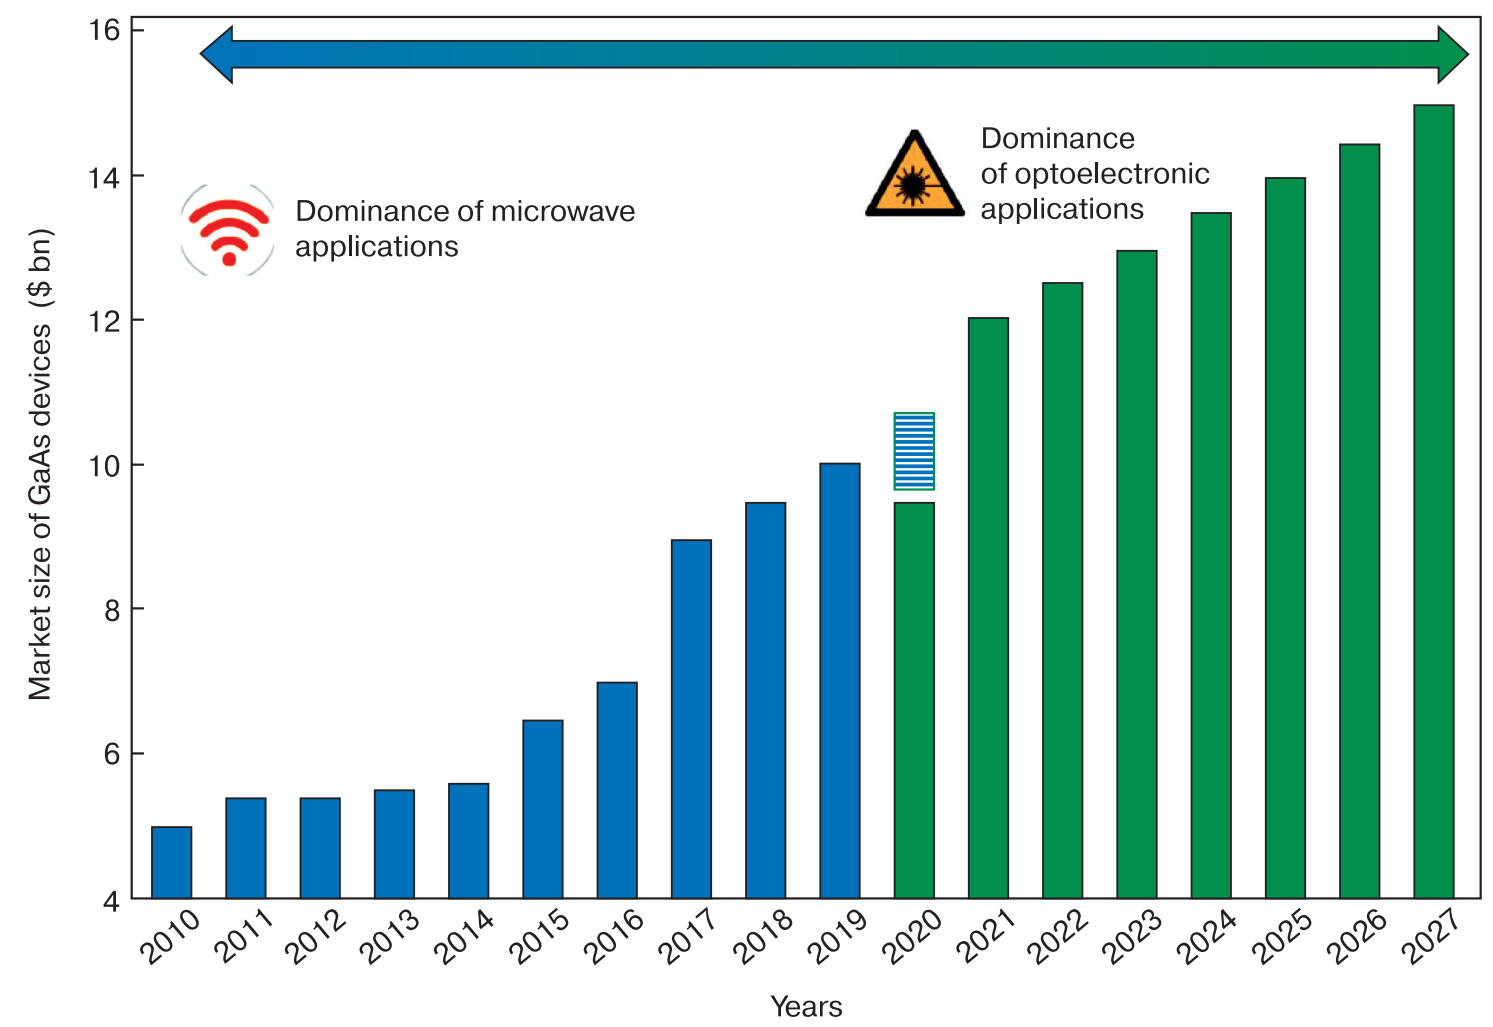
\includegraphics[width=0.8\textwidth]{RisRes}
\caption{\label{figRisRes}
World GaAs device market development and prediction.
Sources \cite{GaAs:Kulch2020}
}%
\end{figure}



GaAs was invented and developed as a basic RF electronics material, but GaAs market development trends are changing now.
The development of photonics and microwave engineering industry has attained a level suggesting
that it will consume most of fabricated GaAs by 2025 \cite{GaAs:Kulch2020}.
In particular, next generation GaAs support the signal speed that is needed to implement 5G \cite{GaAs:MarketAnalys}.
Simultaneously, performance of semiconductor electronic devices is ultimately dictated
by the presence and behavior of point defects.
Therefore detailed knowledge of the properties of those defects under MW irradiation
is crucial to the engineering of robust devices that operate effectively.

Besides, after silicon, GaAs is perhaps the most studied semiconductor.
(Although notwithstanding intense effort over decades, definitive knowledge concerning
even simple intrinsic defects in GaAs remains scanty \cite{EL6:Schultz})
In particular, microwave treatment influence on various parameters of GaAs structure has been investigated
\cite{MW:Rev,ZOHM2000,BHUNIA1998,Bacherikov2003En,Pashkov1994En,
BoltovetsEn,Milenin1994En,BelyaevIntac,ASHKINADZE1996,ProcSPIE,Belyaev1998JTFEn,
Bacherikov2008En,Konakova2015En,Konakova2012FTPEn}.
Consequently, the GaAs is a good model material to study the microwave-induced transformation of defects in semiconductors.


SiC,  a  most  promising  wide  band  gap  semiconductor is widely in use and progress for high power, high-frequency
device applications due  to high saturated electron drift velocity, high mobility,  and  extreme  hardness.
SiC  is  also  a  promising  semiconductor  for  spintronics  and  photonics  due  to  the  spin  coherence
property of some of its lattice defects.
Both 4H and 6H polytypes are the most commonly used hexagonal
polytypes of SiC with wafer size samples and high quality \cite{6HSiC:VV2019}.
4H-SiC is more suitable for manufacturing high-power electronic devices
because of its large forbidden bandwidth, good thermal conductivity, and relatively small anisotropy.
But both 4H- and 6H-SiC are used for power and
opto-electronics, and as growth substrates for graphene and
gallium nitride \cite{SiC:Falk13}.

Moreover, in recent years, point defects in semiconductors have been suggested for implementing quantum bits (qubits)
and single photon sources for quantum computation, quantum information processing, spintronics,
and quantum sensing applications.
Color centers in SiC, such as the silicon vacancy and divacancy,
have recently been shown to be promising qubits for a variety of
applications \cite{6HSiC:VV2019,4HSiC:VV,6HSiC:Singh2021,4HSiC:Vc}.
Point defect qubits may have several nonequivalent configurations with different
characteristics in each polytype which provide alternative tools for engineering qubit properties in SiC.
The theoretical description and engineering of the defect centers
require the assignment of each of the different microscopic configurations.
This has been done for the silicon vacancy and the divacancy in 4H-SiC,
but for 6H-SiC, the work is still in progress \cite{6HSiC:VV2019}.
As a result, nowadays, defects in 6H-SiC are under intensive
investigation \cite{SiC:NV,6HSiC:VV2019,SiC:Falk13,6HSiC:vac2021,SiC:Soltamov21,SiC:Tissot2021,6HSiC:Singh2021,SiCWei}

Thereby now the part of GaAs and 6H-SiC devices is still big enough in industries,
and those materials are promising for future use.
The reviewer is correct, and the use of wide bandgap materials gives the possibility to increase the blocking voltages for high
power devices, as well as to make devices smaller and to reduce power losses.
The reviewer’s suggestion about 4H-SiC and GaN investigation is very interesting, and may be done in the future.

We have added some details in the research justification
(page~2, left column, last paragraph, and right column, fist paragraph).




%In recent years, point defects in semiconductors have been suggested for implementing quantum bits (qubits)
%and single photon sources for quantum computation, quantum information processing, spintronics,
%and quantum sensing applications. The most studied point defect qubits are the negatively charged nitrogen-
%vacancy center (NV center) in diamond, the neutral divacancy in SiC, and the negatively charged silicon vacancy in SiC.
%
%SiC is a technologically mature host for qubits and single photon emitters, which makes it possible
%to integrate quantum technologies and semiconductor devices.
%There are numerous polytypes of SiC which often host multiple symmetrically
%non-equivalent Si and C sites in their primitive cell. Consequently,
%point defect qubits may have several nonequivalent configurations with different
%characteristics in each polytype which provide alternative tools for engineering qubit properties in SiC.
%The theoretical description and engineering of the defect centers
%require the assignment of each of the different microscopic configurations.
%This has been done for the silicon vacancy and the divacancy in 4H-SiC,
%but for 6H-SiC, the work is still in progress.
%
%
%4H and 6H polytypes are the most commonly used hexagonal
%polytypes of SiC with wafer size samples and high quality \сite{6HSiC:VV2019}.
%
%4H- and 6H-SiC,
%the most common hexagonal polytypes, are used for power and
%opto-electronics, and as growth substrates for graphene5 and
%gallium nitride
%SiC:Falk13
%
%
%
%
%-----------------------------
%The excellent material qualities of SiC result in a great potential in applications.
%In addition to the wide range applications of SiC described above, recently the most
%promising area is semiconductor processing.
%Therefore, the use of wide bandgap materials, like SiC, gives the possibility to increase the blocking voltages for high
%power devices, as well as to make devices smaller and to reduce power losses. For switching
%devices, the high saturation drift velocity of carriers in combination with the high breakdown
%voltage, makes the wide bandgap semiconductors superior to most of the common
%semiconductor materials when it comes to impedance matching, output power and switching
%loss. As the power losses are much lower than in silicon, and the thermal conductivity and
%thermal stability are much higher, the need for surrounding cooling system is reduced. Thus,
%in summary, products using wide bandgap electronic devices can be made much smaller and
%much more efficient.
%
%The seeded sublimation growth technique is primarily suitable for the
%production of 4H and 6H-SiC. The largest bandgap in a thermally stable polytype is 3.26 eV
%in 4H-SiC. The saturation drift velocity of carriers is higher in 4H than in 6H-SiC, making the
%propagation of electronic signals faster in 4H-SiC. Therefore there is a strong emphasis on
%studying the properties of the 4H polytype. The technology for growing large pieces of 4H for
%substrate production is also favorable, although the 6H polytype is easier to grow.
%
%This thesis deals with the 4H and 6H polytypes, which are seem to be the most
%promising candidates for future applications.
%----------------------------------------------------
%
%6H ,
%SiC:NV,6HSiC:VV2019,SiC:Falk13,6HSiC:vac2021,SiC:Soltamov21,SiC:Tissot2021,6HSiC:Singh2021,SiCWei
%
%-------------------------------------
%
%Silicon vacancies in silicon carbide have been proposed as an alternative to nitrogen vacancy centers in
%diamonds for spintronics and quantum technologies.
%Optically induced alignment of the ground-state spin sublevels
%of the V−Si in 4H- and 6H-SiC has been demonstrated at room
%temperature [16]. Coherent control of a single silicon-vacancy
%spin and long spin coherence times have been reported [2].
%V−Si are relatively immune to electron-phonon interactions,
%and they do not exhibit fast spin dephasing (spin coherence
%6HSiC:Singh2021
%
%As a promisingmaterial for quantumtechnology, silicon carbide (SiC) has attracted great interest inmaterials sci-
%ence. 4HSiC:Vc
%
%As awide band gap semiconductor, silicon carbide (SiC) plays an important role in the
%power electronics industry owing to its advantages of
%high electronic breakdown field, high thermal conductivity, and chemical stability.
%SiC has different polytypes, of which 3C, 4H, and 6H are themost common ones.Moreover,
%4H-SiC is suitable for manufacturing high-power electronic devices because of its large forbidden bandwidth
%(3.26 eV), good thermal conductivity, and relatively small anisotropy.
%-----------------------------------------------------------------------------------
%
%Color centers in silicon carbide (SiC), such as the negative silicon vacancy (VSi−) and neutral divacancy (VSiVC0
%), have recently been shown to be promising quantum bits (qubits) for a variety of
%applications in quantum communications and sensing.
%4HSiC:VV
%
%In the development of solid-state spin qubits, the nitrogen-
%vacancy (NV) center in diamond is the leading contender.
%Recently, SiC has emerged as a promising platform hosting different
%color centers that emit light near the telecom wavelengths and have
%long spin coherence times, favoring applications in quantum com-
%munications.
%Among these, the negative Si vacancy (VSi−) with zero-phonon lines (ZPLs) at 861.6 nm (V1 center) and 916.5 nm
%(V2 center) in 4H-SiC8 and the neutral divacancy (VSiVC0), i.e.,
%an uncharged complex consisting of a C vacancy (VC)andanearest
%Si vacancy,
%
%---------------------------------------------------------------
%
%It exists in a wealth of different crystal structures with three
%main polytypes: 4H,6H (hexagonal) and 3C (cubic), that
%can be grown in a highly reproducible manner.
%4HSiC:NV
%---------------------------------------------------------------
%
%Silicon  carbide  (SiC),  a  most  promising  wide  band  gap  semi-
%conductor is widely in use and progress for high power, high-frequency
%device applications due  to high saturated electron drift velocity, high
%mobility,  and  extreme  hardness  [1–5].  SiC  is  also  a  promising  semi-
%conductor  for  spintronics  and  photonics  due  to  the  spin  coherence
%property of some of its lattice defects [6,7] and a promising substrate in
%GaN-based  blue  LED  devices  in  optoelectronics  applications
%
%6HSiC:vac2021
%
%
%---------------------------------------------------------------------
%Electron
%spins of the defect center in SiC are excellent candidates for
%quantum information processing and future spin-based quan-
%tum devices.
%SiC:Soltamov21
%-----------------------------------------------------------
%
%Single crystalline SiC is a suitable material for realization of high power, high frequency and high
%temperature devices
%------------------------------------------------------
%---------------------------------------------------------
%
%In order to effectively utilize the photovoltaic properties of gallium arsenide, its surface/interface needs to be properly prepared.
%
%Gallium arsenide is a material widely used mainly in semiconductor technologies
%due to its attractive properties, where it has found many uses.
%In contrast to silicon, it has
%become very popular in high electron mobility transistor (HEMT) structures since it does
%not require any momentum change in the transition between the maximum of the valence
%band and the minimum of the conductivity band, and does not require a collaborative
%particle interaction.
%The direct bandgap of GaAs of 1.42 eV is also
%suitable for diode and photovoltaic (PV) cell applications.
%The advantage of a wide bandgap is also the fact that the material
%remains more semiconductive at higher temperatures, such as in silicon, which has a
%bandgap of 1.12 eV.
%GaAs:Papez2021
%
%----------------------------------------------
%GaAs was
%invented and developed as a basic RF electronics material but GaAs market development trends are changing
%now. The development of photonics and Terahertz (THz)
%engineering industry has attained a level suggesting
%that it will consume most of fabricated GaAs by 2025.
%Requirements to GaAs for MW electronics differ from
%those for photonics and THz engineering by a number
%of important parameters, and their industry development
%principles differ also
%
%In 2019 RF applications reached 33% of GaAs markets by size and 37% by price. GaAs is also widely used in
%optoelectronics as a basic material for LEDs. It seems however that the current GaAs market development trend is
%changing from RF-electronics to photonics.
%GaAs:Kulch2020
%
%Projected manufacturing capacity share of different silicon–based cell technologies. Sources:
%https://www.aleo-solar.com/perc-cell-technology-explained/ (left panel), [1] (right panel).
%-------------------------------------------------------------------------------
%
%
%    Gallium arsenide can be used to manufacture devices such as monolithic microwave integrated circuits, microwave frequency integrated circuits, infrared light-emitting diodes, solar cells, laser diodes and optical windows.
%    GaAs have a direct bandgap unlike many other semiconductors implying it can emit light with high efficiency. Being a direct bandgap material, it is resistant to radiation damage enabling its use in optical windows and space electronics in high power applications.
%    It is also used as an electrical substrate and offers natural isolation between circuits and devices. This makes it suitable for millimeter-wave and microwave ICs.
%    Solar cells based on GaAs power the Opportunity and Spirit rovers that are exploring the surface of Mars. A number of solar cars make use of GaAs in solar arrays.
%    GaAs diodes are used to detect X-rays.
%
%---------------------------------------------------------------------------------------------
%Next generation GaAs support the signal speed that is needed to implement 5G. GaAs works in a way that silicon cannot
%
%https://www.researchandmarkets.com/reports/4991608/gallium-arsenide-gaas-next-generation?utm_source=dynamic&utm_medium=BW&utm_code=q36879&utm_campaign=1358305+-+Gallium+Arsenide+Next+Generation+Semiconductors+Market+Expected+to+Grow+to+%2422+Billion+by+2026&utm_exec=anwr281bwd
%
%-----------------------------------------------------------------------------------
%The interest in high-voltage GaAs structures is due to
%the search for alternative (to silicon) materials for pulse
%power electronics, capable of working at higher pulse repetition rates and higher temperatures. Compared with silicon,
%GaAs has a wider energy gap, substantially higher electron
%mobility (which also exceeds that in SiC and GaN), higher
%dielectric strength, shorter carrier lifetimes, and better radiation hardness. One more advantage of GaAs is that it is a
%direct-band semiconductor material for which solid solutions
%can be obtained, so that the optical and electrical parameters
%of device layers in GaAs–III–V heteroepitaxial structures
%and the electrical characteristics of devices based on these
%structures can be widely varied.
%
%
%Performance of semiconductor electronic devices is dictated
%ultimately by the presence and behavior of point defects. A
%detailed knowledge of the properties and chemical evolution
%of those defects is crucial to the engineering of robust devices
%that operate effectively in normal operation conditions and
%under irradiation.
%After silicon, gallium
%arsenide is perhaps the most studied semiconductor, with
%uses in a variety of devices. Despite early optimism [2]
%and notwithstanding intense effort over decades, definitive
%knowledge concerning even simple intrinsic defects in GaAs
%remains scanty.
%EL6:Schultz




\subsection*{Response to Reviewer \#2 }
\noindent
\textcolor[rgb]{0.00,0.50,1.00}{\textbf{Comment~1.}}
\emph{I suggest the authors concentrating on a specific semiconductor,
digging deeply on the evolution of defects after MWT,
and discussing the effect of doping on the process.
The current work relates to the type of the host,
the single crystal/epitaxial layers, doping concentrations.
Readers lost easily during the introduction of results and discussions.}

\noindent
\textcolor[rgb]{0.51,0.00,0.00}{\textbf{Reply:}}
The various doping concentrations allowed us to conclude 
that the heating and ponderomotive forces are not the main reason 
for the revealed microwave-induced change in the defect subsystem.
The set of GaAs epitaxial structures and single-crystals with different orientations 
allowed the investigation set of various vacancy-related defects
(V$_\mathrm{As}$, V$_\mathrm{As}$As$_i$, V$_\mathrm{Ga}$Ga$_i$V$_{\rm As}$,
V$_\mathrm{Ga}$Ga$_\mathrm{As}$, and V$_\mathrm{Ga}$V$_\mathrm{As}$).
Besides, the difference in dose dependencies in epi-structures and single-crystals
provided additional evidence that dislocation density influences microwave hardness.
Finally, the revealed microwave-induced transformation of 
defects located in the near-surface layer in two materials 
testifies that this phenomenon is typical for semiconductors (at least binary).
The next step after general features research may be deep digging.

To our shame, the reviewer is correct about some fog in Results and discussion. 
We hopefully rephrased the section to add sunlight.





Using two materials 



The text was revised.
In the present paper, we have concentrated on three specific and
common mechanisms, which frequently take place in MSM or MIS structures, and could be
verified experimentally. The reviewer’s suggestion is very interesting, and may be done in the
future.

This is very interesting suggestion, but this comparison requires an additional analysis,
which can be done in the future.
The reviewer’s suggestion is very interesting, and may be done in the
future.

We have added this interpretation in the revised text, in page 11 (second paragraph).
We have revised the text accordingly.
We rephrased this sentence (see page 7)

\vspace{1cm}
\noindent
\textcolor[rgb]{0.00,0.50,1.00}{\textbf{Comment~2.}}
\emph{The authors carried out MWT experiments on differently doped SiC or GaAs.
Did the concentration of dopants change the evolution of point defects?
The Fermi level is different for differently doped hosts,
which charge states of intrinsic defects and MWT-induced defects, and thus the interaction, may be different.}

\noindent
\textcolor[rgb]{0.51,0.00,0.00}{\textbf{Reply:}}
The text was revised.


\vspace{1cm}
\noindent
\textcolor[rgb]{0.00,0.50,1.00}{\textbf{Comment~3.}}
\emph{The Pool-Frenkel effect is related to defect states of dislocations.
Yes, some works dealt the interaction between irradiation-induced point defects and dislocations,
such as Appl. Phys. Lett. 117, 023501 (2020) and J. Mater. Chem. C 9, 3177 (2021).
But I didn’t see any detailed discussion in this work.}

\noindent
\textcolor[rgb]{0.51,0.00,0.00}{\textbf{Reply:}}
The text was revised.

\cite{LightNeuIrrad:1,LightNeuIrrad:2,SiC:bookCh17}


\vspace{1cm}
\noindent
\textcolor[rgb]{0.00,0.50,1.00}{\textbf{Comment~4.}}
\emph{Typos throughout the manuscript should be corrected, including but not limited to:}

\emph{(1) ``and semiconducting compounds including [6, 8]''}

\emph{(2) ``doping degree''}

\emph{(3) ``$0:31\div0:33$''}

\noindent
\textcolor[rgb]{0.51,0.00,0.00}{\textbf{Reply:}}
The text was revised.


\subsection*{Response to Reviewer \#3 }
\noindent
\textcolor[rgb]{0.00,0.50,1.00}{\textbf{Comment~1.}}
\emph{The reviewed manuscript presents results on investigation of deep levels
in various materials before and after microwave treatment with different durations (doses).
Therefore, the investigation is not well focused, since the nature of defects is different
for different materials, and they not necessarily should be governed by the same trends. }

\noindent
\textcolor[rgb]{0.51,0.00,0.00}{\textbf{Reply:}}
The text was revised.


\vspace{1cm}
\noindent
\textcolor[rgb]{0.00,0.50,1.00}{\textbf{Comment~2.}}
\emph{The results could present interest, even though the investigated materials are not the state of the art ones in industries.
However, the used experimental method is not widely approved,
and the identification of the microscopic nature of defects is not an easy
task even with widely used investigation methods such as DLTS or DLOS.
As a result, the discussions about the microscopic nature of the observed defects
and their reconfiguration during the microwave treatment
as well as the made conclusions are not enough convincing
(especially in cases when the deep level activation
energies do not change very much under microwave treatment,
as well as in cases when there is a large difference
between the experimental results and those coming from theoretical consideration).}

\noindent
\textcolor[rgb]{0.51,0.00,0.00}{\textbf{Reply:}}
The text was revised.

\vspace{1cm}
\noindent
\textcolor[rgb]{0.00,0.50,1.00}{\textbf{Comment~3.}}
\emph{I consider that the manuscript is not suitable for publication in the present form.
However, the reliability of the obtained results may be significantly improved,
if the study is complimented with other methods of investigation such as DLTS or DLOS,
at least for some of the investigated materials.
Moreover, the DLTS method also gives information about the concentration of deep levels.
In such a case, a comparison of parameters of deep levels obtained by TAV and DLTS,
combined with an analysis of the results of previously performed investigations,
may provide enough arguments confirming the
proposed microscopic nature of defects and their transformations.}

\noindent
\textcolor[rgb]{0.51,0.00,0.00}{\textbf{Reply:}}
The text was revised.


\section*{References}

\bibliographystyle{iopart-num}
\bibliography{olikh}

\end{document}

